\scanpage{26}
% loc 1, struck NB and words above it
\deleted{\uline{NB} The homomorphism \inserted{of $k$-modules} $A\longrightarrow A\otimes A$ is interpreted as a homomorphism}

% loc 2–4, live NB and definition
\uline{NB} \unsure{To|To} every $k$-module $M$ let us associate the functor in $\unsure{\mathcal O|O|\mathbb O}$-modules
\[
 \unsure{V|\mathbb V|W}(M):\quad k'\longrightarrow\mathrm{Hom}_{k\text{-}\mathrm{Mod}}(M,k')
\]
which depends \unsure{contravariantly} on $M$. We find

% loc 5–7, a) and category map
a) $M\mathrel{\tikz[baseline=-.3ex,x=1em,y=1em]{\draw[line width=.45pt] (0,-.14)--(0,.14) (0,0)--(1,0) (1,-.09)--(1,.09);}}V(M)$ . is fully faithful \unsure{, i.e.,|, i.e.}
\[
 \mathrm{Mod}(k)^{\unsure{0|o|\circ}}\mathrel{\tikz[baseline=-.3ex,x=1em,y=1em]{\draw[line width=.45pt] (0,0)--(1,0) (1,-.12)--(1,.12);}}\mathrm{Mod}(\mathcal O)
\]
% loc 7–8, Hom and cancelled object below
\diagram{\begin{tikzcd}[ampersand replacement=\&,column sep=large]
 \deleted{b)}\quad\forall M,N \& \mathrm{Hom}_{K}(M,N)\arrow[r,"\substack{\alpha_{MN}\\[-2pt]\sim}"] \& \mathrm{Hom}_{\mathcal O}(W(N),W(M))\\
 \& \deleted{\unsure{W(M)(N\otimes{-})|W(M)(N{-})}}\arrow[u,Rightarrow] \&
\end{tikzcd}}
% loc 9, crossed prose before b)
\deleted{\unsure{To see this let us define|To see this define a} homomorphism \unsure{in the opposite direction} $\unsure{f|\varphi}_{M,N}$ \unsure{.}}

% loc 10–11, b) and coupling
b) $\forall M,N$ \deleted{\unsure{$\xi$|:}} the canonical pairing
\[
 V(M)\otimes_{\mathcal O}V(N)\longrightarrow V(M\otimes_k N)\qquad,
\]
% loc 12–14, parenthesis and the smaller writing
\unsure{(|[}which is not an isomorphism, for it is not true that
\[
\begin{aligned}
 &\mathrm{Hom}_{k}(M',k')\otimes_{k'}\mathrm{Hom}_{k'}(N',k')
 \simeq\mathrm{Hom}_{k'}(M'\otimes_{k'}N',k')\quad ]\\
 &\qquad \overset{\unsure{\vee|\sim}}{M}'\otimes_{k'}\check N'\longrightarrow(M'\otimes_{k'}N')^{\vee}
\end{aligned}
\]
nevertheless defines, by taking the $\mathrm{Hom}$ into \deleted{\unsure{$P$}} a $V(P)$, a trifunctorial isomorphism
% loc 15–16, Hom diagram
\margin{\begin{tikzpicture}[x=1mm,y=1mm]\fill (0,0)--(.5,.2)--(1.2,.05)--(1.3,-.4)--(.7,-.8)--(.2,-.65)--(.15,-.25)--(0,-.2)--cycle;\end{tikzpicture}}
\diagram{\begin{tikzcd}[ampersand replacement=\&,column sep=large]
 \mathrm{Hom}_{\mathcal O}(V(M\otimes_k N),V(p))\arrow[r,"\sim"] \& \mathrm{Hom}(U(M)\otimes_{\mathcal O}V(N),V(p))\\
 \mathrm{Hom}_k(P,M\otimes N)\arrow[u,"\sim"'] \&
\end{tikzcd}}
% loc 17–19, On trouve
We therefore find in this way

\textbullet) An $\mathcal O$-linear composition law on a $V(A)$ ($A$ a $k$-module) is a comultiplication $A\overset{\unsure{\pi|\Pi}}{\longrightarrow}A\otimes A$.
% loc 20–22, unité and loi
A \unsure{two-sided|two-sided} unit for the composition law is a \tikz[baseline=(c.base)]{\node[inner sep=1pt](c){counit};\node[anchor=south,inner sep=1pt] at ([yshift=3pt]c.north){\inserted{augmentation}};\draw ([xshift=-2pt]c.south west) to[out=110,in=180] ([xshift=-2pt,yshift=2pt]c.north west) to[out=10,in=180] ([xshift=2pt,yshift=2pt]c.north east);} $A\overset{\varepsilon}{\longrightarrow}k$. \deleted{A} The composition law is associative (commutative) if and only if the algebra law is associative (commutative).

% loc 23–25, Si M and its map
If $M$ is a module, an $\mathcal O$-bilinear pairing $V(A)\times W(M)\mathrel{\tikz[baseline=-.3ex,x=1em,y=1em]{\draw[line width=.45pt] (0,0)--(1,0)--(1,.15);}}V(M)$ is a diagonal map $M\longrightarrow A\otimes M$. \deleted{If} $A$ equipped with a unital $\pi$, then
% loc 25–28, sloping margin note
% slanted
\margin{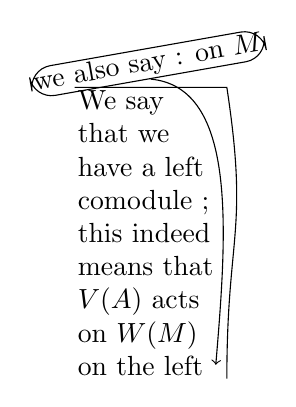
\begin{tikzpicture}[baseline=(m.base)]
 \node[align=left,text width=1.85cm,inner sep=1pt] (m) {We say that we have a \uline{left} comodule ; this \unsure{indeed} means that $V(A)$ acts on $W(M)$ on the left};
 \node[draw,rounded corners=8pt,align=center,inner sep=1pt,rotate=10,anchor=south] (g) at ([yshift=3pt]m.north) {\inserted{we also say : on $M$}};
 \draw[thin] (m.north west) .. controls ([xshift=5pt]m.north west) and (m.north) .. (m.north east) .. controls ([xshift=8pt]m.east) and (m.east) .. (m.south east);
 \draw[->,thin] (g.south) .. controls ([xshift=4pt]m.north east) and (m.east) .. ([xshift=-4pt,yshift=5pt]m.south east);
\end{tikzpicture}}
% loc 26–28, bottom lines
\deleted{law of} the pairing is unital if and only if the diagram \tikz[baseline=(t.base)]{\node[draw,circle,inner sep=1pt](t){$1'$};\fill ([xshift=3pt,yshift=-5pt]t.south east) circle (.7pt);} commutes ; \deleted{If $A$ equipped with a} \inserted{It satisfies} $\mu(\lambda x)=(\lambda\mu)x$ (associativity) if and only if the diagram $2'$ is commutative.
% archive sheet number: 25
